\documentclass[11pt, oneside]{article}   	% use "amsart" instead of "article" for AMSLaTeX format
\usepackage{geometry}                		% See geometry.pdf to learn the layout options. There are lots.
\geometry{letterpaper}                   		% ... or a4paper or a5paper or ... 
%\geometry{landscape}                		% Activate for for rotated page geometry
%\usepackage[parfill]{parskip}    		% Activate to begin paragraphs with an empty line rather than an indent
\usepackage{graphicx}				% Use pdf, png, jpg, or eps� with pdflatex; use eps in DVI mode
								% TeX will automatically convert eps --> pdf in pdflatex		
\usepackage{amssymb}
\usepackage{amsmath}

\title{Continued fractions}
%\author{The Author}
\date{}							% Activate to display a given date or no date

\graphicspath{{/Users/telliott_admin/Dropbox/Tex/png/}}

\usepackage{listings,relsize} 
\lstloadlanguages{R} 
\lstset{language=R,basicstyle=\smaller[1],commentstyle=\rmfamily\smaller, 
  showstringspaces=false,% 
  xleftmargin=4ex,literate={<-}{{$\leftarrow$}}1 {~}{{$\sim$}}1} 
\lstset{escapeinside={(*}{*)}}   % for (*\ref{ }*) inside lstlistings (S code) 
\begin{document}

\maketitle
%\section{}
% \subsection*{R code}
% \begin{lstlisting}  \end{lstlisting}
% \begin{center} 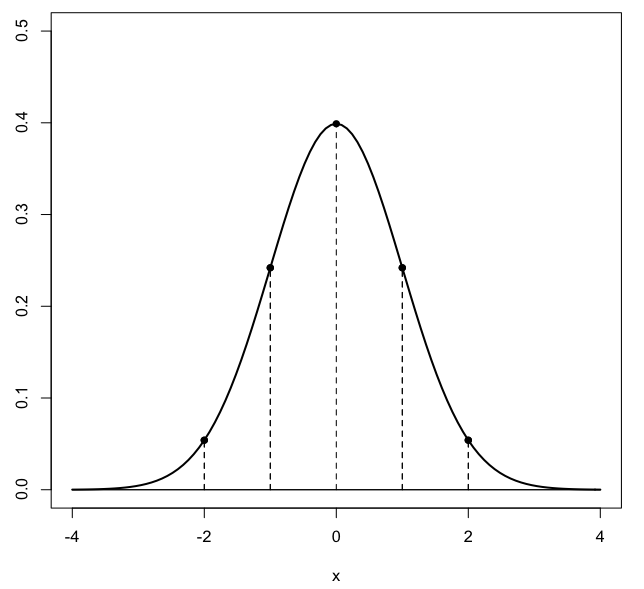
\includegraphics [scale=0.4] {gauss3.png} \end{center}
% \begin{bmatrix} a  &  b \\ c  &  d \end{bmatrix}
% \bigg |_

\large
\noindent
\begin{center} 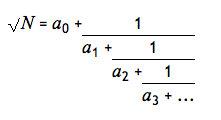
\includegraphics [scale=0.6] {contd_frac.png} \end{center}
According to Problem 64 of  Project Euler, any square root can be written as a continued fraction, in the form shown above.  We'll try first with $\sqrt{23}$ and see if we can find a pattern.  
\subsection*{step 0}
The first part of the method is as follows:  find the next smallest perfect square, in this case $4 \times 4 = 16$.  Now do:
\[ \sqrt{23} = 4 + \sqrt{23} - 4 = 4 + \frac{1}{\frac{1}{\sqrt{23} - 4}} \]
So $a_0 = 4$, and we are ready to start the next stage with the inverse of the fraction we obtained above
\[ \frac{1}{\sqrt{23} - 4} \]
If we generalize this as
\[ \frac{n_i}{\sqrt{23} - d_i} \]
We will be looking for a pattern connecting $n_{i}, d_{i}$ and $n_{i+1}, d_{i+1}$.
\[  a_0 = 4, \ n_0 = 1, \ d_0 = 4 \]
\subsection*{step 1}
At this point, we start the repeating process.  We need to rationalize the denominator 
\[ \frac{1}{\sqrt{23} - 4} = \frac{1}{\sqrt{23} - 4} \ \frac{\sqrt{23} + 4}{\sqrt{23} + 4} = \frac{\sqrt{23} + 4}{23-16} = \frac{\sqrt{23} + 4}{7} \]
and simplify.  In this case we have $4/7 < 1$ and so we do:
\[ \frac{\sqrt{23} + 4}{7} = \frac{\sqrt{23} + 4 + 3 - 3}{7} = 1 + \frac{\sqrt{23} - 3}{7} = 1 + \frac{1}{\frac{7}{\sqrt{23} - 3}} \]
If we just focus on what is under the $1$ in the second fraction we need to work on
\[ \frac{7}{\sqrt{23} - 3} \]
\[  a_1 = 1, \ n_1 = 7, \ d_1 = 3 \]
\subsection*{step 2}
\[ \frac{7}{\sqrt{23} - 3} = \frac{7}{\sqrt{23} - 3} \ \frac{\sqrt{23} + 3}{\sqrt{23} + 3} = \frac{7(\sqrt{23} + 3)}{14} \]
This is where the simplification gets a little trickier, we have another factor in the numerator, $f$.  My hypothesis is that we will always have that $f$ evenly divides into the denominator, as it does here, so..
\[ \frac{7(\sqrt{23} + 3)}{14} = \frac{\sqrt{23} + 3}{2} \]
Now we need to convert this into a form with $\sqrt{23} - n$.  

A second tricky thing is that while we could pull out a $2$ here, in the example, they do $3$
\[ \frac{\sqrt{23} + 3}{2} = \frac{\sqrt{23} + 3 - 3 + 3}{2} = 3 + \frac{\sqrt{23} - 3}{2}\]
The reason is that in the first case, we would have
\[ \frac{\sqrt{23} + 3}{2} = \frac{\sqrt{23} + 3 - 1 + 1}{2} = 2 + \frac{\sqrt{23} - 1}{2}\]
but 
\[ \frac{\sqrt{23} - 1}{2} > 1\]
while
\[ \frac{\sqrt{23} - 3}{2} < 1\]

Finally, we form the continued fraction part (inverting) and have this to go forward with
\[ \frac{2}{\sqrt{23} - 3}\]

At this stage we have:
\[  a_0 = 4, \ n_0 = 1, \ d_0 = 4 \]
\[  a_1 = 1, \ n_1 = 7, \ d_1 = 3 \]
\[  a_2 = 3, \ n_2 = 2, \ d_2 = 3 \]
\subsection*{step 3}
Rationalize
\[ \frac{2}{\sqrt{23} - 3} = \frac{2}{\sqrt{23} - 3} \ \frac{\sqrt{23} + 3}{\sqrt{23} + 3} = \frac{2(\sqrt{23} + 3)}{14} = \frac{\sqrt{23} + 3}{7} \]
Simplify
\[ \frac{\sqrt{23} + 3}{7} = \frac{\sqrt{23} + 3 + 4 - 4}{7} = 1 + \frac{\sqrt{23} - 4}{7}  \]
\[  a_3 = 1, \ n_3 = 7, \ d_3 = 4 \]
Invert
\[ \frac{7}{\sqrt{23} - 4}  \]
\subsection*{step 4}
Rationalize
\[ \frac{7}{\sqrt{23} - 4} \frac{\sqrt{23} + 4}{\sqrt{23} + 4} = \frac{7(\sqrt{23} + 4)}{7} = \sqrt{23} + 4 \] 
Simplify
\[\sqrt{23} + 4 = \sqrt{23} + 4 - 4 + 4 = 8 + \sqrt{23} - 4 \]
Invert
\[ \frac{1}{\sqrt{23} - 4} \]
\[  a_4 = 8, \ n_4 = 1, \ d_4 = 4 \]
\subsection*{Summarizing}
We have
\[  a_0 = 4, \ n_0 = 1, \ d_0 = 4 \]
\[  a_1 = 1, \ n_1 = 7, \ d_1 = 3 \]
\[  a_2 = 3, \ n_2 = 2, \ d_2 = 3 \]
\[  a_3 = 1, \ n_3 = 7, \ d_3 = 4 \]
\[  a_4 = 8, \ n_4 = 1, \ d_4 = 4 \]
At this point, we have the same fraction to work on as what we started with, so we will just repeat the same steps over again.





\end{document}  